%!TEX program = xelatex
\documentclass[a4paper,11pt]{article}
\usepackage[marginparwidth=4.6cm, lmargin=2cm,rmargin=5cm]{geometry}
% \documentclass[twoside, 12pt]{article}

\usepackage{url}
\usepackage{fontspec}
\usepackage{lmodern}
\usepackage{graphicx}
\usepackage[rgb]{xcolor}
\graphicspath{ {../img/} }
\usepackage{marginnote}
\usepackage{polyglossia}
\usepackage{xunicode}
\usepackage{xltxtra}
\usepackage{todonotes}

\renewcommand*{\marginfont}{\footnotesize}

\newcommand{\td}[2][]{
	{\todo[size=\footnotesize]{#2}}
}

\setmainlanguage{czech}

%\usepackage{e-tex}
%\usepackage{etoolbox}
%\usepackage{keyval}
%\usepackage{ifthen}
%\usepackage[czech]{babel}
%\usepackage[backend=biber]{biblatex}
%\usepackage{biblatex}
%\usepackage{polyglossia}
%\usepackage[autostyle]{csquotes}
%\setmainlanguage{english}
%\usepackage{microtype}
%\usepackage[authordate15, backend=biber]{biblatex-chicago}
%\addbibresource{bibl.bib}



\begin{document}

% \pretolerance=1000

\tableofcontents

\section{Úvod}

Různé implementace predikce textu se objevují v mobilních telefonech a elektronických osobních asistentech již přes dvě dekády, přičemž jejich hlavním úkolem je usnadnit zadávání textu na klávesnicích mobilních zařízení. V poslední době se s rozmachem chytrých telefonů objevily systémy predikce textu (a automatické opravy slov, která s ní souvisí) i pro jednoznačné klávesnice typu QWERTY, a to z důvodu zvýšení komfortu psaní. Tyto systémy mají ve většině dvě nevýhody. První z nich je závislost na konkrétním operačním systému, konkrétním zařízení (především v případě starších telefonů) či na konkrétní aplikaci, která zajišťuje zobrazení klávesnice na dotykovém displeji. Takové systémy tudíž nejsou použitelné například pro psaní na stolním počítači na klasické QWERTY klávesnici. Druhou nevýhodou je pak fakt, že systémy musí téměř bez výjimky spoléhat pouze na\td{Jediny, co vim, ze nespoliha na lokalni data, je googlovske rozpoznavani rucne psaneho pisma.. a to je pak nekdy docela blby, kdyz se clovek ocitne na edgi treba} lokálně uložená jazyková data, která tak musí být relativně kompaktní co do datové velikosti a nemusí tedy obsahovat potřebné množství dat, aby uživatel nebyl omezován nedokonalostmi jazykového modelu.

Protipólem velkého množství aplikací pro predikci textu pro mobilní zařízení je pak téměř prázdná množina takových aplikací pro klasické počítače se standardní klávesnicí. Textové procesory typu LibreOffice Writer\footnote{https://www.libreoffice.org/discover/writer/} mívají vestavěné primitivní způsoby doplňování, které ale čerpají data pouze z textu, který je v danou chvíli v editovaném dokumentu. Textové editory typu Atom\footnote{https://atom.io/} mívají podobnou funkcionalitu, navíc například při editaci programového kódu nabízí relativně komplexní doplňování, ale pouze podle předem připravených šablon.

Cílem této práce je tedy vytvořit implementaci systému predikce textu, která bude čerpat data z velkého korpusu textů, a jednak bude jednak nezávislá na platformě. Vzhledem k tomu, že korpusová data není možné uchovávat na straně klienta, bylo logickým krokem zvolit model klienta a serveru, který bude zajišťovat generování predikcí. Tento systém na serveru již v době tvorby této práce existoval, což umožnilo soustředit se především na vývoj uživatelského prostředí. 

Pro zajištění co nejvyšší kompatibility s různými systémy byla zvolena forma zásuvného modulu do webového richtextového editoru CKEditor\footnote{http://ckeditor.com/}. Použitými technologiemi tedy byl především JavaScript pro programovou logiku, AJAX pro komunikaci se serverem a HTML a CSS pro uživatelské rozhraní.

\section{Teoretická část}

Prediktivní text, neboli automatické doplňování textu (angl. autocomplete) je funkce v aplikaci, která na základě uživatelského vstupu (většinou prvních několika znaků slova) doplňuje zbytek části textu (většinou slova). V ideálním případě funkce jednoznačně rozpozná, co chtěl uživatel napsat, a nabídne mu právě to doplnění, jež uživatel chce. V praxi obvykle uživatel dostává na výběr z několika možností, které systém vyhodnotil jako nejpravděpodobnější doplnění vstupu. Systémy se liší způsobem zužování výběru možností a jejich řazením, stejně tak jako vizuálním podáním nabídky.

Všechny systémy automatického doplňování textu fungují nejlépe v implementacích na omezených doménách, tzn. například doplňování e-mailových adres v e-mailových klientech, klíčových slov určitého programovacího jazyka v programátorských editorech či doplňování ve formulářových polích s předem vymezeným očekávaným vstupem. 

Systémy pro predikci textu určené k tvorbě volného textu jsou obvykle založeny na více či méně rozsáhlém lokálně uloženém korpusu slov či slovních spojení, ze kterého vybírají možná doplnění. Tyto systémy zpravidla umožňují uživateli přidávat manuálně slova, která napsal a nejsou v základním korpusu, což slouží jako základní uživatelské přizpůsobení. Lokální korpus má ovšem tu nevýhodu, že jeho velikost je značně limitována možnostmi zařízení, tj. jeho paměťovou a výpočetní kapacitou. To je problém především pro jazyky s rozvinutou flexí, jako je čeština, které potřebují na rozdíl analytických jazyků, např. angličtiny, poněkud větší množství tvarů jednotlivých slov. 

Rozdílnost angličtiny a češtiny v ohledu množství slovních tvarů připadajících na jedno lemma lze porovnat například na dvou velkých korpusech, enTenTen13 a czTenTen12. Jde o rozsáhlé korpusy vytvořené z textů získaných na Internetu, které byly vyčištěny a zbaveny duplikátů nástrojem Onion\footnote{http://corpus.tools/wiki/Onion}. Anglický korpus enTenTen13 obsahuje\td{jak jsem k tomu kurva došel?} 39 011 368 slov a 37 065 442 lemmat (základních slovních tvary). Naproti tomu český korpus czTenTen12 obsahuje slov 18 725 879 a lemmat pouze 13 976 481.\td{doplnit to info z majky o teoretickem pomeru?} V češtině tedy podle výše uvedených dat připadá na jedno lemma 1,339 slovního tvaru, naproti tomu v angličtině na jedno lemma připadá pouze 1,052 slovního tvaru. Je tedy vidět, že slovník pro češtinu by v ideálním případě měl být minimálně 1,27× větší než slovník o stejném množství základních tvarů pro angličtinu.
% cit.: info o korpusech

Tento fakt komplikuje implementaci slovníkových jazykových  modelů do aplikací pro predikci českého textu, protože je nutno uchovávat větší množství slovních tvarů než pro angličtinu. Stejně tak je výrazně větší potřeba\td{ tady by se hodilo neco ocitovat, akorat ze ja jsem si to vymyslel.. nejaky napad?} zohledňovat kontext, aby byly slovní tvary vybírány správně.

\subsection{Klíčové vlastnosti systému pro predikci textu}

Navzdory velmi odlišným způsobům použití systémů pro doplňování textů jsou některé jejich klíčové vlastnosti pro většinu implementací společné. Studie, které zkoumaly efektivitu těchto systémů, obecně docházejí ke podobným závěrům co se požadavků na tyto systémy týče. Ať jde o vyhledávač typu Google nebo Yahoo, o našeptávač e-mailových adres v e-mailovém klientu nebo o predikci volného textu v textovém editoru, aby uživatel měl při užívání aplikace pocit, že mu doplňování textu skutečně pomáhá spíše než překáží, je klíčových několik vlastností.  Primární je rychlost, s níž aplikace možná doplnění uživateli zobrazuje. Nandi a Jagadish uvádí, že by odezva neměla převyšovat 100 ms \cite{Nandi2007}. Tento faktor je rozhodující pro to, zda si uživatel zvolí nabídnutá doplnění použít, nebo raději napíše zbytek textu sám. V případě implementace predikce textu do editoru, kde uživatel zadává volný text, jímž si je relativně jist, je tato vlastnost pro uživatelovo rozhodnutí patrně klíčová. Naproti tomu ve vyhledávání lze očekávat, že uživatel bude ochoten počkat delší chvíli na zobrazení doplnění. S tímto souvisí i další vlastnost, kterou uvádí\td{přehodit jako normalni citaci} Ward a kol. v publikaci Autocomplete as a Research Tool: A Study on Providing Search Suggestions -- umožnění uživateli pohodlně nabízené predikce ignorovat. Rozhodne-li se totiž, že např. bude rychlejší text manuálně napsat a predikce nepoužít, je žádoucí, aby mu grafické zpracování nabídky žádným způsobem neztěžovalo takto učinit. Z tohoto důvodu je ve většině systémů nabídka předvídaných výrazů zobrazována pod textovým polem\td{citace na google suggest? pripadne jak? je to obecne znamy fakt} (např. Google Suggest). 

Zobrazení nabídky v textových editorech, kde se nejedná o jednořádkové pole s očekávaným vstupem pouze několika jednotlivých slov, je předmětem několika studií, z nichž např. jedna navrhuje zobrazovat nabídku na spodní části obrazovky, aby uživatel nebyl nucen přesouvat pozornost příliš daleko od klávesnice. % ocitovat
Lze ale polemizovat nad tím, jak je tato argumentace validní pro uživatele bez motorického nebo jiného postižení, jelikož tací většinou při psaní na klávesnici nehledí. Textové editory pro psaní programového kódu tento problém většinou řeší zobrazováním nabízených doplnění v menu nad nebo pod kursorem (tedy zhruba podobně jako jednořádková vyhledávací a jiná pole). Podobně to řeší i kancelářský balík OpenOffice (příp. LibreOffice), který zobrazuje po napsání prvních tří písmen slova jednu predikci nad kursorem. Výběr predikce se odvíjí od frekvence, přičemž velký důraz je kladen na délku nabízeného slova (obrázek \ref{fig:LOpredict} na straně \pageref{fig:LOpredict}). Tento systém uživateli umožňuje udržovat pozornost na relativně malé oblasti obrazovky, čímž se zvyšuje pravděpodobnost, že se rozhodne doplnění použít. 

\begin{figure}[h]
	\caption{Implementace predikce textu v LibreOffice Writer 4.2.8.2}
	\label{fig:LOpredict}
	\centering
	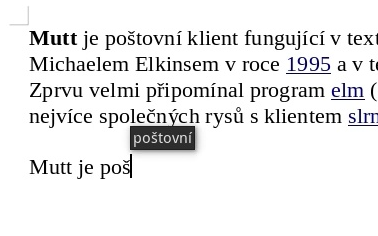
\includegraphics[width=0.7\textwidth]{LO_prediction_1}
\end{figure}

\subsection{Smysl automatického doplňování pro uživatele}

Vedle původního určení predikce textu, kterým je zrychlit zadávání textu a tím komunikaci na rozhraní člověk-počítač, plní pro běžného uživatele automatické doplňování textu ještě několik dalších funkcí. Nejde ani tolik o rychlost zadávání textu, jako spíše o to, co je zadáváno. 

Ward et al. (Autocomplete as a Research Tool) ve své studii uvádí, že studenti, na kterých testoval automatické doplňování ve vyhledávání v rámci informačního systému knihovny, poukázali v následném dotazníku na několik dalších funkcí, které pro ně predikce plnila. 

Na otázku, jak by svým přátelům vysvětlil, k čemu je našeptávač dobrý, odpověděl jeden student, že rozhodně jako asistence v pravopise. Studenti totiž často nemají z ústních zadání v hodinách úplně přesnou představu, jak se např. autor, jehož díla jim jejich vyučující doporučil jako zdroj informací k práci, přesně píše. Autoři studie ze záznamů hledání vyvodili, že někteří studenti si ani nemuseli být vědomi faktu, že začátek jména autora zadali špatně, protože predikce jim nabídla rovnou správnou verzi a oni ji vybrali, aniž by přemýšleli, v čem se nabídka liší od jejich vstupu. 

Mezi další výhody, které studenti uvedli ve výše uvedené studii, patřilo například to, že automatické doplňování jim potvrdilo, že podobné téma již někdo před nimi hledal, a jejich pojetí zpracovávaného tématu je tedy pravděpodobně správné. 

S tímto souvisí i jedna odpověď od dalšího účastníka studie, která uvádí, že autocomplete pro ně fungoval jako nástroj pro dotvoření myšlenky, jako brainstorming od počítače. 

Z výše uvedeného lze tedy vyvozovat, že automatické doplňování textu skutečně nemá význam pouze pro uživatele tělesně či jinak postižené, kteří mohou mít problém se samotným zadáváním textu, ale může posloužit i běžným uživatelům jako nástroj pro kontrolu toho, zda to, co píšou, je správně, k tématu a podobně. [14]

\subsection{Měření účinnosti zadávání textu}

S ohledem na velké množství metod zadávání textu, z nichž mnohé obsahují technologie na ušetření počtu nutných stisků, je nutné mít možnost nějakým objektivním způsobem testovat jednotlivé metody, porovnávat je a zjistit jejich skutečné možnosti. Pro tyto účely slouží metoda výpočtu KSPC (zkratka pro keystrokes per character). Jak název napovídá, udává průměrný počet stisků kláves nutných k zadání jednoho znaku danou metodou\footnote{přestože název obsahuje stisky kláves, veličina se používá i pro měření účinnosti zadávání textu např. pomocí stylusu na dotykovém zařízení}.

Metody zadávání textu lze podle KSPC rozdělit do tří kategorií: ty, pro které je KSPC větší než 1, ty, pro které je rovno 1 a nakonec ty, jejichž KSPC dosahuje hodnot nižších než 1.

Jako základ pro výpočet KSPC pro jednotlivé metody zadávání je vhodná standardní QWERTY klávesnice. Budeme-li uvažovat pouze malá písmena anglické abecedy, platí pro ni, že KSPC = 1, tedy na jeden znak připadá jeden stisk klávesy. Klávesnici QWERTY lze tedy považovat za jednoznačnou metodu zadávání, pro každý znak má jednu dedikovannou klávesu.

Pro další metody zadávání už proces výpočtu tak jednoduchý není a má dva požadavky. Prvním z nich je jednoznačný popis postupu, kterým lze dojít k zadání jednotlivých znaků, druhým je pak jazykový model. Ten je nutný proto, aby výsledné KSPC bylo nezávislé na konkrétním textu v daném jazyce (tedy aby pro daný jazyk bylo průměrné).

\subsection{Jazykový model}

Jazykovým modelem je v tomto případě korpus a jeho omezené formy. Tyto formy se liší podle toho, jaká metoda zadávání je testována. Pokud například jde o metodu, která vybírá znaky nezávisle na kontextu (na okolních znacích), stačí mít informace o frekvenčním rozložení jednotlivých písmen v korpusu. Pokud by byl výběr znaku závislý na kontextu jednoho písmene, byl by jazykový model frekvenční slovník bi-gramů. Pro delší závislosti MacKenzie et al. (2015) použili frekvenční slovník celých slov.

\subsection{Výpočet KSPC}


\[
	KSPC = \frac{\sum{ (K_c × F_c) }}{\sum{ (C_c × F_c) }}
\]

kde $K_c$ je počet úhozů nutný pro zadání znaku, $C_c$ je velikost znaku a $F_c$ je frekvence daného znaku v korpusu. Pokud se tedy tento vzorec aplikuje na situaci, kdy metoda zadávání textu vybírá písmeno bez ohledu na kontext, platí, že $C_c$ = 1, pokud se vybírá v závislosti na jednom předešlém znaku, je $C_c$ = 2. Pokud metoda zohledňuje celá slova, počítá se s průměrnou délkou slov v daném jazyce. Ta se počítá jako vážený průměr počtu znaků ve slovech daného jazyka, který pro BNC vychází na 4,59 znaku; pro srovnání, [15] počítá při svých výpočtech s 5 úhozy na slovo.

\todo[inline]{pokud bych potreboval natahovat, tak tady by se klidne dala dat podkapitola "rozdeleni metod vstupu podle KSPC" - a vykrast MacKenzieho}

\subsection{Technický bláboly okolo predikce}

Problematika predikce textu je intenzivně zkoumána od dob, kdy se rozšířily mobilní telefony s podporou zadávání textu. Jelikož velikost zařízení od začátku nedovolovala osazení plné QWERTY klávesnice, objevovaly se její náhrady, které jsou podrobněji popsány v dalších kapitolách této práce. Jakkoliv se mohla jejich implementace odlišovat, měly obvykle společnou jednu vlastnost, a to nejednoznačnost. Nejrozšířenější se stala klávesnice typu\td{ITU klavesnici mam popsanou nize, mam to nejak linkovat?} ITU, která se udržela dodnes. Tento typ klávesnice sdružuje písmena po třech až čtyřech na jednu klávesu, přičemž ze skupiny se pak vybírá v základním režimu pomocí opakovaných stisků kláves (multitap). Vzhledem k velmi zásadním omezením rychlosti, které tento způsob zadávaní implikuje, byly vyvinuty různé technologie, které se snažily o zrychlení zadávání tak, aby KSPC bylo rovno jedné nebo ideálně menší jedné.

Aby bylo dosaženo KSPC rovného jedné, stačí technologie typu T9, která vyhledává ve slovníku možné kombinacee písmen ze stisknutých kláves a nalezené pak předkládá uživateli. V případě, že existuje ve slovníku pouze jedno slovo, které odpovídá kombinaci písmen ze stisknutých kláves, je dosaženo KSPC rovného jedné. Pokud však takových slov ve slovníku existuje více, je nutno provést výběr a jeho potvrzení, což zvyšuje KSPC nad jedna.

Pro dosažení hodnot KSPC nižších než jedna je už nutné implementovat predikci textu. To znamená, že aplikace musí uhádnout psané slovo ještě dříve, než uživatel napíše všechna písmena daného slova. K tomu, aby mohla účinně předvídat, které slovo uživatel píše, potřebuje kvalitní jazykový model. Jazykový model může být buď slovník nebo statistický model. 

\subsubsection{Slovníkový model}

Pokud systém používá slovníkovou metodu, potřebuje mít k dispozici relativně rozsáhlý frekvenční slovník slovních tvarů a jejich frekvence. Ke slovníku slovních tvarů se obvykle přidává ještě frekvenční slovník n-gramů, který zajišťuje účinnější predikce díky zohlednění kontextu. Pokud například tedy implementace využívá slovníku bi-gramů, je pak teoreticky aplikace, která je na ní postavena, schopna předvídat nejen doplnění slova, která uživatel zrovna píše, ale i celá slova, která by mohl chtít napsat po dokončení předchozího slova.

Frekvenční slovník je slovník, který ke každému heslu uvádí hodnoty spojené s frekvencí daného slova ve zdrojovém korpusu. Obvykle to je hodnota absolutní frekvence daného slova a například Frekvenční slovník češtiny %  cit. Čerák et al. 
uvádí také průměrnou redukovanou frekvenci, což je hodnota, jež vychází z absolutní frekvence, avšak zohledňuje rozložení daného slova v korpusu. Pokud tedy mají dvě slova stejnou frekvenci, avšak první z nich se vyskytuje pouze v malém množství odborných textů, zatímco výskyty druhého jsou rovnoměrně rozloženy přes celý korpus, druhé slovo dostane vyšší číselnou hodnotu ARF než slovo první. Podle hodnoty ARF tak lze vyvodit, že druhé slovo je obecně známější a užívanější širším publikem. %  cit. Frek slovník, Čermák, předmluva 
V kontextu s predikcí slov to může například znamenat, že je pravděpodobnější, že uživatel chce napsat spíše druhé slovo nežli to první, které je pravděpodobně značně odborné.

Tvorba frekvenčních slovníků byla v dobách před rozvojem počítačů schopných zpracovat velká množství textů poněkud komplikovaná. Vzniklé databáze bylo obtížné aktualizovat, jejich výroba byla náročná a pomalá. Nástup počítačů však většinu těchto problémů odstranil, takže je možné velmi snadno z korpusu vyrobit frekvenční slovník, který bude tak aktuální, jako je samotný korpus. Na rozdíl od ručního zpracování dat navíc počítačové zpracování dovoluje pracovat s mnohem většími korpusy, takže výsledný frekvenční slovník může být i přesnější. Pro srovnání, jeden z prvních frekvenčních slovníků pro angličtinu,\td{jeste by to chtelo nejaky data o soucasnych frekvencnich slovnicich, nebo staci ty priklad o BNC? Prip. kde je vzit? } The Teachers Word Book of 30,000 words, měl 30 tisíc lemmat (z 13 tisíc slovních rodin %  cit. Goulden, Nation and Read, 1990 
) a byl vyroben z ručně psaného korpusu, který obsahoval 18 milionů slov. %  cit. http://www.lextutor.ca/research/nation_waring_97.html 
Naproti tomu Britský národní korpus (BNC) má 112 milionů tokenů a webový korpus enTenTen (2013) má tokenů téměř 23 miliard. %  cit. sketch engine 

\todo[inline]{a sem asi nekam patri, ze se taky data berou z uziv. dat - gmail}

Implementace frekvenčních slovníků v aplikacích pro predikci textu se pravděpodobně značně liší a vzhledem k tomu, že jde o uzavřené komerční systémy, není možné konkrétní implementace zjistit.

\subsubsection{Statistický model}

\todo[inline]{A tady si budu muset jeste neco vymyslet... a nejdriv si to nastudovat}

% Odlišný způsob, jak uchovávat data o jazyce, je využívat statistického modelu, který obsahuje data o n-gramech a jejich frekvencích, neboli pravděpodobnostech. Takový model pak negeneruje predikce z předem daného seznamu slov, ale ze seznamu n-gramů. Jeho výhodou je vyšší flexibilita, protože nemusí vůbec znát výsledné slovo na to, aby například správně desambiguoval pravděpodobně zamýšlený význam klávesy na nejednoznačné klávesnici. Vzhledem k tomu, že statistický model může být relativně úsporný co se datové náročnosti týče, 

% Nevýhodou je, že systém, který využívá statistický model s n-gramy obsahujícími jen kupříkladu dvojice písmen, může předpovídat před


\subsection{Historie predikce textu}

Původním smyslem automatického doplňování bylo usnadnit zadávání textu uživatelům s fyzickým postižením, aby museli provést menší počet stisků kláves pro napsání požadovaného textu. Brzy se však ukázalo, že funkce automatického doplňování je užitečná pro široké spektrum uživatelů, kteří často zadávají např. dlouhé technické či medicínské termíny, pro vyplňování formulářů a pro zařízení, která disponují nejednoznačnou klávesnicí, jako jsou mobilní telefony, tedy klávesnicí, kde jedna klávesa zastupuje více znaků. 

Poslední případ byl zvláště důležitý, protože na zmíněných klávesnicích bylo např. pro napsání slova „nejlepsi“ bylo bez prediktivního textu nutno stisknout 17 kláves, naproti tomu s prediktivním textem stačilo kláves pouze 8. \cite{dXVv6nPb2KifFXYv}

\subsection{Typy predikce textu podle využití}

\subsubsection{ITU klávesnice}

Predikce textu se historicky vyskytovala v mnoha podobách, jež obvykle závisely na použití daného softwaru, typu zařízení (především velikosti obrazovky či typu klávesnice a podobně) a cílové skupině uživatelů. První systémy pro predikci textu se vyskytovaly u mobilních telefonů s numerickými klávesnicemi, na nichž byly jednotlivým klávesám přiřazeny skupiny písmen tak, aby jejich počet vyšel na počet numerických kláves. Původní patent na plně funkční prediktivní vstup na telefonní klávesnici pochází z roku 1985, publikován byl v roce 1988 \cite{Feinson1988}. Byl určen pro uživatele s poruchou sluchu a počítá s telefonním přístrojem řízeným mikroprocesorem, jenž poté, co uživatel zadá dostatečný počet znaků, aby mohla ve slovníku být nalezena jednoznačná shoda, zobrazí na displayi CRT nalezené slovo, které uživatel následně vybere.

Technicky podobné přístupy se vyskytovaly i u pozdějších mobilních telefonů s numerickými klávesnicemu typu ITU (klávesnice podle normy E.161) \cite{mfmtlqoxL48pMk3T}, které byly využívány na psaní krátkých zpráv, správu kontaktů nebo např. vyhledávání na WAP. 

Na těchto\td{sem bych dal nejakou ukazku z te ceske wiki} klávesnicích musel uživatel stisknout klávesu s požadovaným písmenem tolikrát, jaké bylo pořadí daného písmena na klávese. Například na klávese 3 jsou písmena D, E, F, tudíž chtěl-li uživatel zadat písmeno F, musel klávesu 3 stiknout třikrát. Tento systém zadávání se nazývá multitap. Při psaní tímto systémem mohlo KSPC dosahovat hodnot přes 2 \cite{dXVv6nPb2KifFXYv}, protože většina kláves musela být stisknuta vícekrát než jednou. 

Z těchto důvodů se začaly objevovat technologie, které měly proces psaní zjednodušit. Většina z těchto systémů predikce textu pracovala na základě analýzy uživatelova vstupu a porovnávání se slovníkem. Alternativním řešením bylo použítí databáze skupin písmen, které se vyskytují v daném jazyce, pro který je model určen, z nichž pak lze skládat požadovaná slova.

\subsubsection{T9}

\td{overit, jen si nejsem jist jak..} Nejrozšířenějším systémem pro predikci textu na klávesnicích typu ITU byl systém T9, akronym pro Text on 9 keys, vyvinutý společností Tegic Communications \cite{Edq6tEyjOSzk54RQ} patentovaný ve Spojených státech \cite{Grover1998}. Systém T9 umožňuje uživateli zadávat text stiskem každé klávesy pouze jednou, nikoliv několikrát, jako je tomu u klasického zadávání způsobem multitap. Systém potom vyhledává ve slovníku záznamy korespondující se sekvencí stisknutých kláves, tzn. slova, která obsahují písmena ze stisknutých kláves. 

Většina implementací umožňovala uživateli přidávat k vestavěnému slovníku do takzvané uživatelsky definované databáze (User Defined Database, UDB) nová slova pomocí předdefinované klávesy. Množství slov ve slovníku pak záviselo na konkrétní implementaci. Novější implementace navíc řadily slova podle frekvence užívání, což zajištovalo, že častěji používaná slova z n-tice slov psané stejnými klávesami byla nabízena jako první. 

Taková slova, která se zapisují stiskem stejných kláves, se nazývají textonyma \cite{ZORN2007} a jsou jimi v angličtině např. slova „book“ and „cool“. Zatímco obvykle tento jev pouze snižuje efektivitu zápisu pomocí T9, v roce 2010 záměna dvou textonym v textové zprávě vedla ve Spojených státech k vraždě. \cite{bjjL0GPb5QxyO1A8} 

Jednou z hlavních výhod systému T9 je schopnost automatického doplňování textu po zadání prvních několika písmen ze slova. Systém po napsání prvního písmene obykle začne nabízet nejfrekventovanější slova začínající na dané písmeno a nabídku upravuje podle dalších stisknutých kláves. Některé implementace se také jsou schopny naučit nejpoužívanější dvojice slov a po napsání prvního slova z některé z dvojic nabídne systém automaticky další slovo, které uživatel může přijmout stiskem předdefinovaného tlačítka. \cite{hrzQ70bvKjUBgVml} 

Další funkcí, která je pro uživatelské pohodlí důležitá, je schopnost rozpoznat a opravit překlepy. T9 toto činí tak, že se dívá i na přilehlé klávesy, tzn. pokud uživatel chce napsat slovo „testing“, které lze zapsat klávesami {\tt 8378464}, ale stiskne místo toho sekvenci kláves {\tt 8278464}, systém T9 mu stejně nabídne vedle slova „tasting“ i slova „testing“ a „tapping“ \cite{hrzQ70bvKjUBgVml}.

\subsubsection{iTap}

iTap je systém konkurenční k systému T9 vyvinutý firmou Motorola. Přestože oba systémy plní rámcově stejnou funkci, a to pomoci uživateli při psaní textových zpráv na klávesnicích typu ITU, a oba využívají slovníku pro nabídku doplnění, liší se v přístupu k uživatelskému prostředí. Slovník pro systém iTap obsahuje kromě jednotlivých slov i běžně užívané fráze.
% chybi citace

Zatímco T9 je kontextově nezávislý systém, iTap uživateli nabízí doplnění v závislosti na kontextu. Uživateli pak je prezentována nabídka možných slov, která se v kontextu nachází. 
%chybi citace, to jsem asi vytahal ze sve pameti.. 

Jedna studie \cite{lBNMeL7t9XcnqSzq} uvádí, že ve srovnání se systémem iTap je systém T9 pro uživatele výhodnější v tom smyslu, že nejsou nuceni činit rozhodnutí ohledně toho, zda v určitém momentu zvolit nabízenou predikci, či pokračovat v manuálním psaní. Pro nezkušené uživatele navíc může u systému iTap být demotivující, když jim predikce nabídne slova, které nemínili napsat. Systém iTap je také celkově mírně náročnější na ovládání.

\subsubsection{LetterWise}

LetterWise je systém prediktivního psaní vyvinutý a patentovaný firmou Eatoni Ergonomics. Jeho distinktivním rysem oproti ostatním systémům pro psaní na klávesnicích typu ITU je fakt, že nepracuje se slovníkem, ale s databází pravděpodobností prefixů pro každý používaný jazyk. Které písmeno ze stisknuté klávesy zvolit tedy systém vybírá porovnáním pravděpodobností, s jakými mohou písmena z dané klávesy následovat po předcházejících již zadaných písmenech. V angličtině je například nepoměrně pravděpodobnější, že po sekvenci písmen T a H bude následovat při stisku klávesy 3 písmeno E, nikoliv D či F. Prediktivní systém LetterWise má tedy v paměti zařízení uloženy pouze tyto pravděpodobnosti, nikoliv celá slova. \cite{MacKenzie2001} To jej činí zajímavým oproti ostatním slovníkovým systémům ze dvou důvodů.

Prvním z nich jsou nízké paměťové nároky. Databáze pravděpodobností prefixů v praxi zabírá v zařízení mezi\td{tady by se hodilo doplnit, kolik ma slovník pro T9, ale to se mi nepodarilo zjistit .. a hlavne ocitovat ty zatraceny byty, bo od toho se mi ta citace nekde zatoulala} 500 a 9000 byty pro každý jazyk.

Druhým, pro uživatele výrazně citelnějším důvodem, je možnost relativně jednoduše zapisovat i neslovníková slova. Pokud se uživatel pokouší totiž zadat slovo, které by sice ve slovníku neexistovalo, ale má skladbu hlásek odpovídající jazyku, jehož databázi prefixů používá, je pravděpodobné, že systém vybere správné písmeno. Další vlastností implicitně vyplývající z faktu, že systém nepoužívá slovník, je, že se uživatel nikdy nemusí uchylovat k zápisu slov klasickým způsobem (tedy že stiskne klávesu 3 dvakrát, chce-li zadat písmeno E). Při zápisu slov, jejichž posloupnost písmen se nepodobá jazyku databáze, musí uživatel pouze v případě špatného odhadu následujícího písmena stisknout klávesu pro volbu dalšího písmene. Tento systém tedy uživatele nenutí v případě zjištění, že jím požadované slovo není ve slovníku, celé slovo smazat a zadat jej klasickým způsobem. \cite{MacKenzie2001} \cite{Ghayoomi2009}

\subsubsection{WordWise}

Firma Eatoni Ergonomics společně se systémem LetterWise vyvinula ještě jeden méně známý systém - WordWise. Ten je na rozdíl od systému LetterWise založený na doplňování slov ze slovníku, v čemž je podobnější systému T9. Na rozdíl od něj ale, ve chvíli, kdy uživatel chce zadat slovo, které není obsaženo ve slovníku aplikace, nenutí uživatele zadat vlastní slovo multitap způsobem, ale vrací se k systému LetterWise. U něj, jak jsme uváděli výše, záleží počet nutných stisků kláves na podobnosti slova s právě používaným jazykovým modelem. 

Modifikací tohoto systému je také systém WordWise Shift, který využívá jednu klávesu na telefonu, které není přiřazeno žádné písmeno, jako klávesu Shift, a na každé klávese se skupinou písmen je vybráno jedno písmeno, které lze napsat pouze se stiskem klávesy Shift a dané klávesy. Toto má podle výrobce za cíl minimalizovat problémy s predikcí slov, která sdílejí stejnou kombinaci kláves. Společnost Eatoni na svých stránkách uvádí, že uživatel při používání tohoto systému nemusí vůbec sledovat display svého zařízení, a přesto bude může jím napsaný text být zcela správně, protože chyba v predikcích slov nastává jednou za 440 slov. \cite{Ward2012} 

\subsection{QWERTY klávesnice na smartphonech}

V posledních letech se s rozvojem smartphonů s velkými dotykovými obrazovkami začínají dostávat do širšího používání plné QWERTY klávesnice (případně národní modifikace jako česká QWERTZ, které pro jednoduchost budou zahrnovány v rámci této práce pod pojem QWERTY klávesnice, jelikož se liší jen rozložením znaků a přidanými národními znaky). 

Pokud by se účinnost klávesnice jako metody vstupu textu porovnávala pouze podle hodnoty KSPC, byly by plné QWERTY klávesnice na smartphonech stejně účinné jako standardní klávesnice k počítačům. Realita je ovšem jiná, protože vzhledem jednak k velikosti klávesnic na smartphonech, která je místo desítek centimetrů na šířku v řádu centimetrů, a jednak k tomu, ze na rozdíl od fyzické klávesnice nejsou jednotlivé klávesy rozpoznatelné po hmatu, vyžaduje zadávání textu na takové klávesnici ze strany uživatele větší zkušenosti a pozornost. Text navíc nemůže zadávát všemi deseti prsty, ale při nejlepším dvěma prsty, což rychlost zadávání také rapidně snižuje. Nemožnost poznat hranice kláves po hmatu navíc vede k zásádnímu nárůstu chybovosti (překlepů), které je uživatel nucen opravovat. Ačkoliv je pravděpodobně nereálné snažit se bez empirického výzkumu zahrnout tyto faktory do výpočtu teoretického výpočtu KSPC pro tyto klávesnice, lze logickým úsudkem dospět k tomu, že i pro tuto metodu vstupu je žádoucí zvýšit rychlost a účinnost zadávání nějakým typem predikce textu.

\subsubsection{Barevné zvýrazňování kláves}

Jedním z navrhovaných způsobů, jak pomoci uživatelům snížit množství překlepů při psaní na QWERTY klávesnicích bez haptické odezvy, bylo bareveně odlišovat nejpravděpodobnější následující klávesy. \footnote{http://web.ist.utl.pt/~daniel.j.goncalves/research/paelife\_textentry/paelife\_textentry.html} Tento způsob byl navržen především pro starší uživatele, kteří jednak nemusejí být seznámeni s rozložením QWERTY klávesnice, a jednak nemají takovou přesnost motoriky a rychlost reakcí, jako uživatelé mladí. 

Klávesy byly odlišeny různými odstíny šedivé barvy, a to lineárně podle toho, jak pravděpodobné bylo dané písmeno v souvislosti s předchozím zadaným znakem. Vedle barevného odlišení pozadí klávesy byl ještě zvětšen popisek klávesy.

\todo[inline]{nejaky cisla a obrazek z toho clanku }

Výsledky zmiňované studie, která byla provedena na 15 ženách a 5 mužích ovšem předpoklad, že to starším uživatelům pomůže, popřely. Ukázalo se, že snaží-li se klávesnice vizuálně nějakým způsobem odlišit prvky a přitáhnout k nim pozornost uživatele, působí to na něj spíše rušivě a výrazně to snižuje rychlost zadávání textu. 

\subsubsection{Predikce celých slov}

\td{tady by to rozhodne chtelo citaci, ale nevim, jak si ji vyfabrikovat --predelat citaci} Druhým navrhovaným způsobem ve výše zmíněném článku byla metoda, kterou používá v současné době většina klávesnic na smartphonech. 

Jde o systém, kde po zadání znaku či znaků je ze slovníku známých slov vybráno několik slov, která jsou v souvislosti s již zadanými znaky nejpravděpodobnějšími řetězci, jež uživatel chce zadat. Tento seznam je obvykle nabízen ve formě horizontálního seznamu nad klávesnicí a uživatel může ušetřit několik stisků kláves tak, že vybere požadované slovo ještě před tím, než jej celé dopíše (za předpokladu, že jej systém našel ve svém slovníku a správně navrhl). 

Oproti zvýrazňování jednotlivých nejpravděpodobnějších kláves má tento systém minimálně dvě výhody. Jednak nevyžaduje, aby si uživatel nestínil svými prsty, kterými píše, výhled na klávesnici, a jednak uživateli zobrazuje celá slova, ne pouze další znak z nich. % cit Neveřilová Ulipová, pg 14

Nevýhodou této metody na druhou stranu je fakt, že je na uživatele kladena vyšší kognitivní zátěž v tom smyslu, že je nucen procházet zrakem seznam navrhovaných slov a přemýšlet, zda je mezi nimi i to, které zamýšlel napsat. Z tohoto důvodu je nutné délku seznamu návrhů omezit na optimum - některé práce uvádí, že ve své implementaci používají 6 návrhů.

\subsubsection{Swype}

Další systém zadávání textu, který je poněkud odlišný od všech dosud zmíněných, je tzv. Swype. Jde o systém původně vyvinutý firmou Swype Inc., nyní vlastněný a vyvíjený firmou Nuance Communications, určený výhradně pro dotyková zařízení. Uživatel v něm nezadává text ťukáním na jednotlivé klávesy, ale přejíždí prstem či stylusem po klávesnici od prvního písmena zadávaného slova k poslednímu tak, aby na cestě přejel pokud možno přes všechna písmena obsažená ve slově. % http://www.cnet.com/news/move-over-t9-here-comes-swype/ a http://www.swype.com/product-features/android/features.html

Swype se skládá ze tří základních částí - analyzátoru trasy dotyku, systému na vyhledávání slov ve databázi výrazů a uživatelského prostředí. V raných verzích databáze obsahovala\td{damn.. tady mi zase utekla citace nekam do haje} 65 000 výrazů.

Nutno podotknout, že firma Nuance, jež systém Swype vyvíjí, nezahrnuje do své klávesnice pouze tento systém zadávání, ale i klasickou metodu zadávání s nabídkou predikcí v horizontálním seznamu. Navzdory faktu, že hlavním důvodem popularity klávesnicové aplikace Swype je systém zadávání Swype, i klasické klávesnice v této aplikaci kombinují různé technologie na zlepšení uživatelského pohodlí. Mezi ně patří například schopnost rozšiřovat virtuální (nikoliv vizuální) velikost klávesy podle toho, jaké klávesy předcházely. Pokud uživatel tedy např. často tapne na klávesu N, smaže zadaný znak N a tapne na klávesu B a pokračuje v psaní, pak se to klávesnice naučí a příště, pokud je tapnutí ne zcela jednoznačné, vybere pravděpodobnější klávesu, v tomto příkladu tedy B. % http://www.swype.com/product-features/android/features.html 

% http://www.nuance.com/ucmprod/groups/corporatecomms/@web-enus/documents/webasset/nc\_024737.pdf

Swype používá Andvance Language Model (AML), „pokročilý jazykový model“, který pracuje s bigramy a trigramy vytvořenými mimo jiné na základě textů, které už uživatel zadal. To aplikaci umožňuje účinněji desambiguovat slova, která vychází jako možná řešení uživatelova vstupu. AML také umožňuje předvídat další slovo, které by uživatel mohl chtít zadat, pomocí [/ how the fuck am i supposed to know .. aka edit this /].

\subsubsection{Predikce na fyzických QWERTY klávesnicích}

Jak bylo naznačeno v kapitolách výše, většina implementací predikce textu, automatického doplňování textu a automatických oprav založených na predikci textu je určena pro zařízení buď s nejednoznačnou klávesnicí, kde má za cíl zjednodušit a zrychlit zadávání textu eliminací nutnosti několikanásobného stisku klávesy pro zadání jednoho znaku, nebo pro zařízení s dotykovou obrazovkou, na níž je zobrazována virtuální klávesnice, kde sice teoretická hodnota KSPC je rovna jedné, ale absence haptické odezvy klávesnice způsobuje vyšší chybovost při zadávání textu. 

Existují ale případy, kdy je predikce textu vhodná i pro použití s klávesnicemi fyzickými. Lze usuzovat, že se tyto případy nebudou týkat uživatelů, kteří nemají motorický handycap a jsou na fyzickou QWERTY klávesnici zvyklí, ale spíš uživatelů, kteří z nějakého důvodu nemohou zadávat text normální rychlostí. Takoví uživatelé většinou trpí nějakým typem omezení motoriky rukou, a tudíž nejsou schopni rychlého pohybu prstů po klávesnici. Pro takové uživatele má predikce textu smysl v tom, že nemusí zadávat celá slova, ale stačí zadat jeho menší část a poté vybrat požadované slovo z nabídky předvídaných slov, což pro ně patrně bude jednodušší, než muset zadávat celá slova. Taková predikce textu může napomoci např. lepší sociální interakci těchto uživatelů, protože rychlost komunikace může být značnou překážkou v účinné výměně informací s protistranou, která takovým handycapem netrpí, a nemá tudíž například trpělivost čekat na odpověď v chatu nadstandardní dobu. %  nejaky citace? jako nekde jsem neco podobneho cetl, ale buh vi kde..   


Proto jsme se rozhodli v rámci této práce implementovat systém prediktivního textu, který se zaměří na automatické doplňování delších slov (doplňování krátkých slov obvykle účinnost zadávání nezvyšuje, protože počet stisků kláves nutný k výběru daného slova nebude nijak výrazně nižší než počet stisků kláves nutný k manuálnímu doplnění daného slova) s důrazem na eventuální schopnost navrhovat na základě již zadaných slov možné další výrazy. Druhým základním požadavkem na tuto implementaci je jednoduchá použitelnost uživatelského prostředí, které by nabízené výrazy mělo zobrazovat neobtruzivním způsobem a umožňovat uživateli z nich jednoduše vybírat.

\section{Praktická část}

Jak bylo naznačeno v úvodu, cíl této práce leží v úmyslu pokusit se implementovat tradiční, byť poněkud zjednodušený, model automatického doplňování textu pro uživatele s fyzickou QWERTY klávesnicí s tím, že na rozdíl od tradičních systémů popsaných v práci výše nebude mít tato aplikace lokální slovník nebo databázi n-gramů, ale vešekeré operace produkující možná doplnění budou prováděny na vzdáleném serveru.

Základní výhodou tohoto modelu je fakt, že na vzdáleném serveru, na němž se provádí všechny operace spojené s analýzou vstupu a tvorbou predikcí, je možné skladovat výrazně vyšší množství jazykových dat, které slouží jako databáze známých slov. Při implementaci predikce textu a automatického doplňování na straně klienta je totiž nutno počítat se značně omezeným datovým prostorem, nehledě na to, že mnohé klienty stále nemají výpočetní výkon dostatečný k rychlému prohledávání extrémně velkých textových korpusů.

Při umístění jazykových dat na vzdálený server je sice nutno počítat s neustálým připojením k internetové síti, na druhou stranu nutno uznat, že v implementaci určené pro klasické počítače, která je součástí této práce, by to neměl být omezující faktor. 

\subsection{Analýza}

\subsubsection{Backend}

Zde popisovaná aplikace je závislá na serverovém skriptu, který tvoří takzvaný backend. Tento backend byl, společně s předchozími verzemi popisované aplikace, vyvinut již dříve a zcela nezávisle na této práci. 

V této práci je tedy backendem skript naprogramovaný v dynamickém programovacím jazyce Python, který s webovou aplikací komunikuje pomocí protokolu CGI. 

Jako zdrojová data pro skript produkující doplnění slouží předem vygenerované n-gramy o délce\td{proc jich je tolik, kdyz to stejne funguje jenom s bigramama? } 3 až 12 tokenů. Tyto n-gramy pochází z nejrozsáhlejšího českého korpusu czTenTen, který je kolekcí textů z různých webových zdrojů. Texty v korpusu neprošly korekturami, takže nemusí nutně obsahovat pouze spisovnou češtinu, což může být závažným problémem, pokud by aplikace pro predikci textu měla být využíváná pro kontrolu správnosti psaní. Vzhledem k tomu, že ale není primární cíl, nebyl na tuto skutečnost během vývoje aplikace brán zřetel. 

% cit. https://ske.fi.muni.cz/auth/corpora/

Vygenerované n-gramy byly pak vyfiltrovány podle různých kritérií s cílem vytvořit databázi n-gramů, která bude mít přijatelné pokrytí textů korpusu se zachováním rozumné datové velikosti databáze.

% konec parafraze clanku neverilova+ulipova::ch3.1, to se asi cituje jinak, ze?}

\todo[inline]{tady jeste popsat neco o tech FSA}[-2cm]

\todo[inline]{prostor pro popis, jak se ty n-gramy vazi}

Vstupem skriptu ve zde popisované implementaci jsou poslední dvě slova z textového editoru na frontendu. Serverový skript pracuje v základu ve dvou režimech, a to v závislosti na tom, zda vstup, který dostává, končí mezerou, či nikoliv. Pokud končí mezerou, předpokládá se, uživatel poslední slovo vstupu dokončil a chystá se psát další, pokud mezera na konci vstupu není, je rozumné předpokládat, že uživatel slovo ještě nedokončil a chystá se v něm pokračovat. Podle tohoto jsou také rozdělené režimy, ve kterých serverový skript pracuje. 

V prvním případě, tedy pokud na konci vstupu mezera je, jsou jeho výstupem nejpravděpodobnější celá slova, která se v bigramech vyskytovala za slovem, které je posledním slovem vstupu. Pokud mezera na konci vstupu není, výstupem skriptu jsou slova, která se v bigramech vyskytovala na pozici za předposledním slovem vstupu a zároveň začínají řetězcem, který je shodný s posledním (nedokončeným) slovem na vstupu. Je důležité si povšimnout, že výstupem nejsou pouze doplnění posledního nedokončeného slova,ale celá slova obsahující i vstupní řetězec. Tímto se druhý režim odlišuje od prvního, který vrací doplnění, která lze jednoduše připojit za text bez nutnosti odstraňovat část v editoru již existujícího textu.

Co se formy vstupu a výstupu týče, má tento serverový skript velmi jednoduché rozhraní. Vstupní řetězce přijímá přes HTTP požadavek, v němž jsou data přenášena metodou GET, tedy jako parametry URL, například {\tt http://nlp.fi.muni.cz/projekty/predictive/predict.py?input=sk\%C3\%A1kal+pes+}. Vstupem je v uvedeném příkladu tedy {\it skákal\_pes\_} (podtržítka značí mezery). Jelikož posledním znakem je mezera, očekávaným výstupem budou slova, která lze doplnit za {\it pes}. 

Skript pak vrací aplikaci, z níž byl požadavek odeslán, text (zobrazitelný jako stránka v prohlížeči) s maximálně 13 doplněními, která jsou oddělená mezerou.

Díky tomuto jednoduchému konceptu komunikace tedy stačí, aby aplikace, která serverového skriptu využívá, byla schopna odesílat HTTP požadavky na konkrétní URL adresu. 

\subsubsection{Frontend}

Cílem této práce bylo vyvinout zásuvný modul do webového editoru CKEditor, což je textový HTML editor, jehož cílem je zjednodušit produkci obsahu pro webové stránky. Editor umožňuje pracovat s pokročilým formátováním ve značkovacím jazyce jazyce HTML (HyperText Markup Language), který se používá pro tvorbu webových stránek a webového obsahu. Práce s formátováním je založena na principu WYSIWYG, což znamená, že uživatel nemusí mít žádné znalosti HTML, protože pro aplikaci formátování lze použít vizuální prvky ve formě tlačítek a rozbalovacích menu, podobně jako v klasických kancelářských textových procesorech typu LibreOffice Writer nebo Microsoft Office Word.

CKEditor je open source aplikace, což znamená, že jeho zdrojový kód je veřejně přístupný a každý jej může libovolně modifikovat, používat a distribuovat za dodržení jistých podmínek. 

Výhodou CKEditoru je jeho modularita, která spočívá v možnosti rozšiřovat jej pomocí zásuvných modulů. Tvorba zásuvných modulů není vyhrazena pouze pro vybrané autory, ale  díky otevřenosti kódu editoru se jí může zabývat takřka kdokoliv. Proto je CKEditor vhodným výběrem pro účely této práce. %  cit. http://ckeditor.com/about 

\subsection{Návrh}

Jelikož výsledkem práce je zásuvný modul do webového HTML editoru CKEditor, byly při vývoji využity výhradně webové technologie, tedy JavaScript v kombinaci s knihovnou AJAX (asynchronní JavaScript a XML), značkovacím jazykem HTML (HyperText Markup Language) a kaskádovými styly (Cascading Style Sheets, CSS). 

\subsubsection{JavaScript}

JavaScript (JS) je dynamický, interpretovaný, objektově orientovaný programovací jazyk široce využívaný pro vývoj webových aplikací. Z hlediska komunikačního modelu klient-server se jedná o jazyk pro skriptování na straně klienta, takže se používá pro programování uživatelského rozhraní webových stránek. % cit. https://developer.mozilla.org/en-US/docs/Web/JavaScript/About_JavaScript 


Jeho vývoj, který probíhá od roku 1995 dodnes, začal ve společnosti Netscape Communications Corporation pod jmény Mocha a LiveScript jako doplněk programovacího jazyka Java pro amatérské programátory. V roce 1997 se JavaScript stal průmyslovým standardem poté, co Ecma International, mezinárodní nevýdělečná organizace pro normalizaci komunikačních systému, vydala první standardizovanou verzi JavaScriptu pojmenovanou ECMAScript. %  cit. https://en.wikipedia.org/wiki/JavaScript --vytahat primarni zdroje 

Ve zde popisovaném zásuvném modulu slouží JavaScript k obstarání hlavní logiky rozhraní, tedy extrakci textových dat editoru a jejich zpracování do formy vhodné k odeslání serverovému skriptu, sledování aktivity uživatele a případné zajištění, že data budou odeslána. Po přijetí odpovědi serveru zpracovává JavaScript přijatý text, zajišťuje uživateli nabídku doplnění a jejich případně vložení na správné místo v editoru. 

\subsubsection{AJAX}

AJAX, neboli Asynchronous JavaScript and XML, je souhrnné označení webových technologií, které se používají pro vývoj webových aplikací. Hlavním využítím AJAXu bývají právě aplikace, které potřebují komunikovat se vzdáleným serverem bez nutnosti načítat celou webovou stránku znova. 

Asynchronní výměna dat se serverem probíhá pomocí aplikačního rozhraní XMLHttpRequest (XHR), které skriptovacím jazykům na straně klienta, jako je například JavaScript, umožňuje odesílat data na vzdálený server. Po přijetí odpovědi se pak stará od dodání dat zpět do skriptu.

Pro komunikaci se serverem se využívá vzhledem k velmi malým objemům dat, které je nutno přenášet, prostého textu, a to ve dvou formách. První z forem se používá při odesílání požadavku, kde jsou data serveru dodávána v rámci URL jako parametry. Jedná se vždy o posledních několik slov (záleží na konfiguraci skriptu na klientově straně), která jsou zakódována globální funkcí JavaScriptu {\tt encodeURI}, aby byla zajištěna správná funkčnost i v případě výskytu zvláštních znaků, jako jsou například písmena s diakritikou nebo jakékoliv jiné znaky, které v URL adrese být přímo nemohou. Jednotlivá slova jsou oddělována pomocí znaku {\tt +}, který je v URL adrese může nahrazovat mezeru.Druhá forma prostého textu se využívá v odpovědích serveru. Skript na požadavky odpovídá textovým řetězcem, který obsahuje navrhovaná slova oddělená mezerou. Tento textový řetězec je odesílán klientu jako dokument obsahující prostý text, který neobsahuje žádné přídavné strukturní nebo designové prvky, takže je opět velmi snadno zpracovatelný.

\todo[inline]{nejaky schema typu "klient odesle serveru url se slovama, server to zpracuje a odesle uzivateli text"? }

\subsubsection{jQuery}

\todo[inline]{Popisovat?}

\subsubsection{HTML}

HTML, neboli HyperText Markup Language je standardní značkovací jazyk velice podobný jazyku XML široce používaný pro tvorbu webových stránek pro webové prohlížeče, jako je kupříkladu Mozilla Firefox či Google Chrome. Webové prohlížeče jsou schopny HTML zpracovat a zobrazit uživateli výslednou stránku, která obsahuje vizuální prvky a textové formátování. 

Standard HTML vychází ze obecného značkovacího jazyka SGML (Standard Generalized Markup Language), který je založen na dvou principech, a to že by značkovací jazyk měl být deklarativní, tedy popisovat strukturu a další atributy spíše než definovat způsob, jakým je dokument zpracováván, a že by definice v dokumentu měly být jednoznačné a pevně definované, aby byl dokument zpracovatelný stejně jako například programový kód. %  cit. https://en.wikipedia.org/wiki/Standard_Generalized_Markup_Language --vytahat primarni zdroje, budou-li 


HTML popisuje strukturu stránky po sémantické stránce, stejně jako definuje (částečně či úplně) její vzhled. Rozdíl mezi sémantickou informací a informací pouze o tom, jak by měla prezentace vypadat, lze ilustrovat na dvojici značek, jejichž výsledná prezentace je zpravidla identická, a to {\tt <strong>} a {\tt <b>}. Značka {\tt <strong>} webovému prohlížeči říká, že text uvnitř této značky je důležitější než okolní text a měl by podle toho také být naformátován (tedy zpravidla tučným řezem písma), zatímco značka {\tt <b>} pouze indikuje, že by text v ní uzavřený měl být naformátován tučně. %  cit. https://en.wikipedia.org/wiki/HTML --primarni zdroje?? 


Zde popisovaná aplikace využívá HTML relativně málo, protože se jedná o zásuvný modul, který ze své podstaty nesmí ovlivňovat vzhled stránky, do níž si uživatel vloží CKEditor s tímto modulem. V rámci editačního pole se však vyskytla potřeba HTML použít pro zobrazení nabídky s výběrem jednotlivých možných doplnění, z nichž si uživatel může vybrat. Jakkoliv tedy co do množství kódu je HTML zastupováno nejmenší částí ze zde popisovaných technologií, je jeho použití důležité pro komfort koncového uživatele.

\subsubsection{CSS}

Druhou technologií, která je relativně málo využita, ale pro koncového uživatele je zásadní z hlediska uživatelské přívětivosti rozhraní, jsou kaskádové styly (CSS). CSS je také jednou ze základních technologií používaných pro webové prezentace a zajišťuje definice vizuálního vzhledu stránek napsaných ve značkovacím jazyce.

Hlavním smyslem CSS je oddělení obsahu webové stránky od její vizuální prezentace. To je důležité jednak pro snazší udržování stránky, a jednak to přispívá k přehlednějšímu zpracování zdrojového kódu. Použití CSS navíc umožňuje zobrazit jednu stránku různými způsoby, jedním z nichž může být například možnost zobrazení pro barvoslepé uživatele.

Ve zde popisované aplikaci je tedy CSS využíváno k definici vizuální prezentace nabídky alternativních doplnění.

\subsection{Implementace}

\subsubsection{Uživatelské rozhraní}

Mluvit o uživatelském rozhraní jako celku je v tomto případě poněkud problematické, protože jde o zásuvný modul a není tudíž možné předvídat, jak přesně bude koncový uživatel modulu mít CKEditor nakonfigurován. Pro účely této práce však postačí uvažovat základní konfiguraci CKEditoru tak, jak je poskytována na oficiálních webových stránkách. Tam jsou k disposici ke stažení předpřipravené tři balíčky, jež se liší množstvím zásuvných modulů, které jsou obsahují. Pro účely vývoje zde popisovaného pluginu i pro účely samotného popisu\td{sem se mi hrozne nehodil ten pasiv.. ale - je to spatne? neni? ja nevim popravde} jsme vybrali nejmenší balíček {\it Basic Package}, který obsahuje 17 zásuvných modulů obstarávající základní formátování. V popisu uživatelského rozhraní pak bude uvažována webová stránka, na níž se bude nacházet pouze CKEditor v konfiguraci {\it Basic Package} s přidaným pluginem, který je předmětem této práce.

\todo[inline]{zde nekde screenshot editoru}

Práce v takto nakonfigurovaném editoru probíhá tak, že uživatel zadává text do editoru pomocí klasické klávesnice a vybírá si (případně nevybírá) doplnění, která jsou mu v průběhu nabízena. Doplnění jsou nabízena vždy, když na určitou dobu přestane vyvíjet aktivitu (pro účely testování se jako vhoné ukázalo být 300 ms), a když jsou pro danou kombinaci slov a písmen před pozicí kursoru nalezena doplnění. Pokud nalezena nejsou, nabídka se nezobrazuje. Ve chvíli, kdy si uživatel některé doplnění z nabídky vybere, skript jej v závislosti na situaci vhodným způsobem doplní do editoru, přidá za nově doplněné slovo mezeru a posune na její místo kursor. Pokud uživatel poté nevyvine žádnou další aktivitu po 300 ms, zobrazí se mu další doplnění zvolené na základě předchozího slova zadaného (či vybraného) slova. V ideálním případě by tak mělo na základě prvního slova být možné doplnit určité standardní věty pouhým vybíráním vhodných\td{tomu ale brani to nastaveni, ze filtrujeme kratky slova, bo nema smysl je nabizet} predikcí. 

\subsubsection{Zpracování textu v editoru}

Aby mohla být serverovému skriptu odeslána data, na jejichž základě budou vyhledána možná doplnění, musí být na straně klienta zpracován text, který uživatel napsal do editoru. To probíhá v několika krocích, jejichž výsledkem je řetězec předem definovaného počtu posledních slov v editoru, který je vhodný k odeslání na server.

Všechny operace spojené s modifikacemi textu v editoru i prezentací nabídky predikcí prováděny pouze v případě aktivity uživatele. Touto aktivitou se myslí\td{JavaScriptove -- jak se to pise, kdyz je to adjektivum? mne je nejak proti srsti to napsat s malym j a velkym S xD} JavaScriptové události {\tt keydown} a {\tt keyup}, které reprezentují stisky kláves -- konkrétně stisknutí klávesy ({\tt keydown}) a její uvolnění ({\tt keyup}).

Prvním krokem je rozdělení obsahu editoru na jednotlivá slova. To zajišťuje funkce {\tt sliceContent()}, jež přijímá text editoru ve formě řetězce (datový typ String). Text rozděluje postupně na řádky podle tagu {\tt <br>}, kterým končí v CKEditoru každý řádek, a dále zpracovává pouze poslední řádek. To sice znemožňuje používat predikci na jiném než posledním řádku, což ale nevadí, protože momentálně celkově plugin nepodporuje práci s predikcemi na jiných místech než na úplném konci vkládaného textu. To je jeden ze známých nedostatků, který bude rozebrán ve vyhodnocení. Následně funkce HTML tagy odstraní, nahradí nedělitelné mezery normálními a rozdělí zpracovávaný řádek na jednotlivá slova. Jako datový typ pro uložení řetězce rozděleného na slova bylo zvoleno pole (Array) pro velké množství operací, má v jazyce JavaScript připraveno. Další operace prováděné funkcí {\tt sliceContent()} na výsledném poli jsou\td{jak se spravne rika to, ze to jsou proste nepodstatny blbosti, kteryma spravuju ruzny divny chovani CKEditoru? xD } čistě technického rázu. 

Poté, co má skript k dispozici slova z aktuálního (posledního) řádku v editoru, se v případě, že současné slovo u kurzoru má délku alespoň tři znaky, zjišťuje, zda se v editoru už nevyskytuje slovo, které začíná na řetězec shodný se současným slovem a má délku alespoň pět znaků. Pokud ano, přidá se do seznamu predikcí, který později bude uživateli nabídnut. Tento krok se provádí proto, že lze předpokládat, že pokud uživatel napsal jednou nějaké delší slovo a znova začal psát slovo, které začíná stejnými znaky, bude chtít napsat téže slovo. Jde o funkcionalitu podobou té z textového procesoru LibreOffice Writer.

Po tomto kroku už přichází na řadu funkce {\tt getSuggestions()}, která provádí AJAXové volání na server za účelem získání predikcí vytvořených z korpusových dat. Funkce {\tt getSuggestions()} přijímá několik hodnot, a to pole se slovy z posledního řádku, počet slov, která mají být odeslána na server a dále callback na funkci {\tt handleSuggestion()}, která zpracovává získaná doplnění.

Ve funkci {\tt getSuggestions()} pak proběhne připravení řetězce se slovy, která mají být odeslána na server. To znamená, že funkce metodou {\tt slice()} vyřízne z pole posledních N slov, kde N je počet slov odesílaných na server a výsledné pole N prvků spojí do řetězce s tím, že mezi jednotlivé prvky pole, tedy slova, vloží znak {\tt +} (plus). Znak {\tt +} byl zvolen proto, že slova jsou odesílána, jak již bylo popsáno v kapitole Návrh, metodou GET, tedy jako parametry adresy URL, a v rámci dat odesílaných metodou GET lze reprezentovat mezeru buď znakem {\tt +} nebo řetězcem {\tt \%20}, přičemž tyto způsoby jsou v praxi rovnocenné.

Nyní funkce čeká předem nastavenou dobu, zda nenastane další aktivita uživatele, a v případě, že nenastane, odešle AJAXový požadavek na server. Tento požadavek má velice jednoduchou formu, jak již bylo uvedeno výše, jedná se pouze o zavolání URL a předání řetězce se slovy, jenž byl připraven výše uvedeným způsobem, formou požadavku GET.

V případě, že AJAXové volání na server uspělo (návratový kód 202 (Success)), zavolá se díky callbacku, který byl funkci {\tt getSuggestions()} předán dříve, funkce {\tt handleSuggestion()}. Pokud volání z jakéhokoliv důvodu skončilo chybou (příkladem budiž nedostupný server, což způsobí, že volání skončí návratovým kódem 404 (Not Found)), vypíše se chyba do konsole a z hlediska uživatele se nic nestane. 

Funkce {\tt handleSuggestion()} přijímá jako argumenty mj. současné slovo pod kursorem, jedno doplnění z existujícího textu v editoru a odpověď serveru. Odpověď serveru je řetězec znaků, který obsahuje slova oddělená od sebe znakem {\tt <TAB>}. 

Základním předpokladem při vývoji zde popisované aplikace je fakt, že tento systém bude využíván uživatelem, který má nějakou potíž při vkládání textu pomocí klasické QWERTY klávesnice. Proto návrh počítá s tím, že není smysluplné nabízet slova kratší než tři znaky, protože výběr takového slova ze seznamu nabízených predikcí vyžaduje přibližně stejný počet stisků kláves, jako napsat samotné slovo. Vzhledem k tomu, že úprava serverového skriptu tak, aby splňoval tento požadavek, by mohla ztížit jeho využití v jiné aplikaci, se filtrování slov provádí až na straně klienta. Proto funkce handleSuggestion() poté, co obdrží pravděpodobná doplnění současného slova v editoru, případně slova, která by mohla následovat, filtruje doplnění tak, aby mezi nimi byla pouze taková, která jsou delší, než předem zadaná délka (tedy čtyři znaky). Tím vzniká seznam slov, do něhož stačí doplnit případná doplnění, která byla nalezena v již existujícím textu v editoru, aby bylo možno jej prezentovat uživateli.

\subsubsection{Zobrazení predikcí}

Nabídka predikcí sestává ze dvou různých částí. První z nich je predikce (jíž může být celé slovo po mezeře, či část slova doplňující již zadanou část slova v editoru), která se zobrazuje méně výrazným typem písma topograficky ihned za zadávaným textem v hlavním editoru. Takové doplnění lze přijmout pouhým stiskem tabulátoru. Tento způsob doplnění je inspirován technologií Google Suggest, která funguje na podobném principu. 

Pro tento způsob zobrazení predikce je využíváno tzv. stínového editoru, který je pomocí CSS umístěn přesně pod hlavní editor, v němž uživatel zadává text, a do něhož je pomocí JavaScriptové funkce {\tt copyContent()} ve zde popisovaném zásuvném modulu kopírován text z hlavního editoru. Pro zobrazení predikce je pak využíváno toho, že text zkopírovaný z hlavního editoru má ve stínovém editoru identické prostorové vlastnosti jako text hlavního editoru a lze na jeho konec snadno připojit aktuální predikci, která se tak zobrazuje uživateli fontem stínového editoru, který v případě zde popisované implementace má šedou barvu (předpokládá se, že text v hlavním editoru má černou barvu). 

Vzhledem k tomu, že predikce nejsou vždy dokonalé nebo není možné jednoznačně rozhodnout, které slovo uživatel zamýšlí napsat, ukázalo se být nutným zobrazovat i alternativní predikce. 

Tyto alternativní predikce jsou prezentovány pod pozicí kursoru ve formě seznamu. Pokud chce uživatel vyžít některou predikci zobrazenou v seznamu, stačí mu opětovně stisknout klávesu tabulátor, s jejíž pomocí lze v seznamu jednosměrně cyklovat mezi položkami. Aktuální položka se pak zároveň kopíruje do hlavního editoru, takže po dosažení požadované predikce uživatel stiskne klávesu mezerník a může pokračovat v psaní. Tato metoda volby byla navržena především s ohledem na původní cíl aplikace, tedy usnadnit psaní uživatelům, kteří z mají z nějakého důvodu problém zadávat text na QWERTY klávesnici. Cílem tedy není zrychlení psaní, jako tomu bývá u implementací prediktivního textu například pro dotyková zařízení, ale co nejvíce snížit množství stisků různých kláves pro volby predikce.

Nabídka alternativních predikcí je zobrazována vždy pod kursorem, aby uživatel nebyl nucen dělit svou poroznost na různá místa obrazovky. O zobrazení nabídky v místě kursoru se stará funkce showAlternatives(), která je závislá na funkci getSelectionCoords(). Z pohledu problematiky implementace je zajímavá především funkce getSelectionCoords(), která pomocí zjišťování pozice aktuálního výběru textu získává pixelovou pozici kursoru, jež je nutná pro správné zobrazení alternativ. Implementace výběrů je velmi závislá na konkrétním prohlížeči, avšak lze obecně říci, že aktuální výběr vždy končí v místě, kde je právě umístěn kursor. S ohledem na tuto skutečnost a na to, že API moderních prohlížečů umožňuje získat pixelové pozice začátku a konce výběru lze pak pixelovou pozici výběru považovat za pixelovou pozici kursoru, na níž se má zobrazit nabídka alternativních doplnění. 

Výběry mají v aplikaci ještě další způsob využití, a to přesunutí kursoru na korektní místo poté, co je vložena zvolená predikce. Je zřejmé, že kursor nemůže zůstat na původním místě, na němž byl před vložením predikce, protože pak by uživatel buď psal další text před vloženou predikci, nebo by musel manuálně přejít na konec vkládaného textu. Tento problém je sice snadno řešitelný přemístěním kursoru o délku predikce dále, ale v praxi se ukazuje, že existuje nezanedbatelné množstí případů, kdy výběr není korektně umístěn v textu a tudíž ani pozice kursoru na jeho umístění závislá není správná. Je to způsobeno především odlišnou a nedokonalou implementací v různých prohlížečích, protože nejde o standardizovanou součást API prohlížečů. Zajistit tak například korektní umístění kursoru při vkládání predikce nikoliv na konec, ale doprostřed textu, se ukázalo být velice\td{nejsem si uplne jist, jak moc zabihat do podrobnosti o selections a tehle vecech, protoze jejich vysvetleni pro filozofy by mohlo byt docela obtizne.. a vlastne pro vsechny, protoze je to dost silena vec} problematické, a proto od toho v rámci této práce bylo upuštěno. 

\subsubsection{Vkládání predikcí}

Ve verzi zásuvného modulu rozebírané touto prací jsou vybrané predikce do textu vkládány na úplný konec řetězce znaků v hlavním editoru. Úplným koncem je myšlen viditelných znaků, tedy vyjma HTML značek a konce řádku.

V případě vkládání celého slova, nikoliv doplnění zbytku již zadaného slova, je vložení predikce relativně triviální. Jde pouze o připojení dané predikce za mezeru na konec již existujícího řetězce znaků. 

Ovšem v případě doplňování pouhé části slova jde, vzhledem k tomu, že serverový skript i v tomto případě vrací celá slova, nikoliv jejich příslušné části, o úkon, který obsahuje zásah do již existujícího textu. Pokud tedy uživatel napíše jako poslední slovo řetězec „p“ a předcházející slovo je „vážený“, navrácená slova jsou „paciente“, „pane“, etc. Je tedy zřejmé, že nelze zvolenou predikci (např. „paciente“) vložit přímo za existující text, ale je nutné nejdříve začátek slova, pro který je predikce určena, smazat, a pak až predikci vložit. Tento problém je řešen smazáním již napsané části slova z predikce, jejíž zbytek je pak vložen za napsaný text. Do hlavního editoru se tedy nevkládá celá predikce „paciente“, nýbrž pouze její zbývající část po odtržení již napsané části, tedy „aciente“.

Z hlediska plynulosti práce se tento způsob ukázal být vhodnější než mazání již vložené části slova z hlavního editoru a vkládání celé predikce na jeho místo, mimo jiné proto, že se pozice kursoru přitom mění pouze jednou, nikoliv dvakrát.

\subsection{Vyhodnocení}

Při testování hotového zásuvného modulu se projevilo několik probémů, jejichž obrysy byly naznačeny v předcházejícíh kapitolách. 

\todo[inline]{ tady by to chtelo nejake pojednani o tom, ze vlastne cilem bylo dosahnout KSPC < 1, coz jsem tam nikde nemel}

Cíl práce, tedy vyvinout aplikaci, která by umožňovala zadávání textu bez nutnosti stisku všech kláves korespondujících s písmeny ve slovech zadávaného textu, byl splněn. Pokud uživatel chce zadat text, jehož slova existují v korpusu, z něhož jsou vybírány predikce, má možnost z těchto predikcí vybrat vhodně ty, které odpovídají jeho záměru, a snížit tak KSPC na hodnotu menší než jedna. Vzhledem k velikosti korpusu, z něhož jsou predikce vybírány, je rozumné předkládat, že takového výsledku lze dosáhnout téměř s libovolným textem v českém jazyce. Současná implementace navíc umožňuje snížit počet stisknutých kláves na počet znaků v textu také tím, že mezi predikce zařazuje již zadaná delší slova. Tato funkcionalita může být užitečná například pro uživatele, kteří zadávají odborný text s větším množstvím dlouhých odborných termínů (dobrým příkladem budiž lékařské texty).

Dalším využitím tohoto zásuvného modulu může být případ, že text zadává uživatel, který si není jist správným psaním jednotlivých slov. Po zadání začátku slova mu jsou prezentovány varianty slova, které na dané pozici mohou být, a uživatel si z nich může vybrat, aniž by byl zběhlý v morfologii a syntaxi českého jazyka. K tomuto bodu je však nutno podotknout, že korpus, jehož data jsou zdrojem k tvorbě predikcí, má za zdroj texty publikované na Internetu, které neprošly korekturami, a tudíž se u nich nelze spoléhat na gramatickou správnost. Pokud by tedy zde popisovaná aplikace měla být primárně určena uživatelům, jejichž rodným jazykem není čeština, bylo by nutné zdrojové texty zkontrolovat a zajistit tak jejich gramamtickou správnost.

Co se problémů týče, hlavním z nich je fakt, že momentální implementace neumožňuje práci vprostřed těla textu, ale pouze na jeho konci. Není tak možné mít text, do jehož části chce uživatel vložit odstavec, ve kterém by využíval predikce textu, protože se způsob, jakým je momentálně algoritmus vkládání navržen, umožňuje pouze na úplném konci textu. Zde je tedy značný prostor pro zlepšení, a to hlavně v případě, že se zlepší implementace výběrů textu v prohlížečích.

\todo[inline]{tady by bylo na miste zminit naprostou neschopnost podporu formatovani textu, ale to az pokud zjistime, ze to nejsme schopni spravit.. stejne jako to vraceni kursoru na spravne misto, pokud ma text vic jak jeden odstavec.. bylo by docela trapne, kdybychom tohle tam museli nejak vysvetlovat xD (teda ja, lol)}

\subsection{Závěr}

\begin{figure}[h]
	\centering
	
\includegraphics[width=0.7\textwidth]{daria}
\end{figure}
\section{Zdroje}

%\nocite{*}
%\printbibliography
\bibliographystyle{ieeetr}
\bibliography{bibl}


\end{document}
